%%%%%%%%%%%%%%%%%%%%%%%%%%%%%%%%%%%%%%%%%%%%%%%%%%%%%%%%%%%%%%%%%%%%%%%%%%%%%%%%
%	TRABAJO: Proyecto Integrador
%		Titulo: 	Desarrollo de IP cores con procesamiento de Redes de Petri 	
%					Temporales para sistemas multicore en FPGA					
%		Autores:	Juli�n Nonino												%					Carlos Renzo Pisetta										%		Director:	Orlando Micolini											
%%%%%%%%%%%%%%%%%%%%%%%%%%%%%%%%%%%%%%%%%%%%%%%%%%%%%%%%%%%%%%%%%%%%%%%%%%%%%%%%

% Path im�genes: ./marco_teorico/redes_de_petri/img
% Nombre predeterminado im�genes: petrixx
%	xx es el numero de imagen

\section{Clasificaci�n de las Redes de Petri}
	\label{sec:clasificacion}

	Las \textbf{\emph{Redes de Petri (PN)}} se pueden considerar como aut�matas formales y generadores de lenguajes formales. En las siguientes secciones, se analizar�n un conjunto de sintaxis restrictivas que limitan el poder de modelado de las Redes de Petri pero permiten asegurar que el modelo generado cumple con ciertas propiedades.
	\begin{figure}[H]
		\centering
		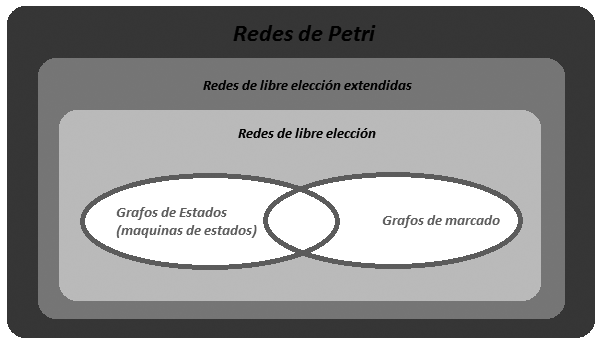
\includegraphics[width=1\linewidth]{./marco_teorico/redes_de_petri/img/Petri08}
		\caption{Subclases de Redes de Petri}
		\label{fig:Petri08}
	\end{figure}
	
	\subsection{Grafos o m�quinas de estado}

		Para representar una m�quina de estados con una Red de Petri, se deben cumplir las siguientes condiciones: cada transici�n tiene un �nico arco de entrada y un �nico arco de salida, las plazas no tienen restricci�n y solo existe un token en toda la red. Esto significa que no puede existir concurrencia, pero si puede haber conflictos. Los conflictos se deben a que como una plaza puede tener muchos arcos de salida, no se puede determinar hacia donde ir� un token. Por ejemplo, en la Figura \ref{fig:Petri09} un token en la plaza $P0$ generar� conflicto entre las transiciones $T0$ y $T1$ dado que no se puede determinar cual debe ser disparada.
		\begin{figure}[H]
			\centering
			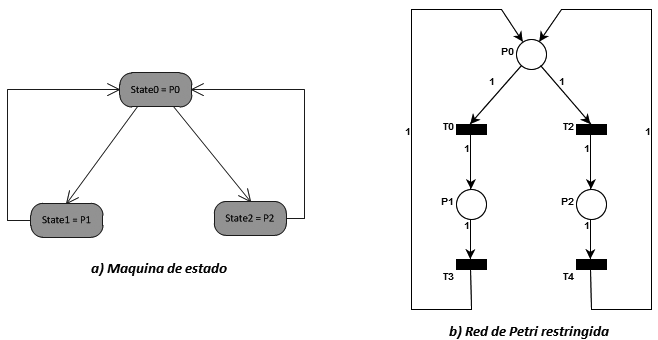
\includegraphics[width=.8\linewidth]{./marco_teorico/redes_de_petri/img/Petri09}
			\caption{Red de Petri restringida a m�quina de estados}
			\label{fig:Petri09}
		\end{figure}
		
		Matem�ticamente, sea $t$ una transici�n perteneciente al conjunto de transiciones $T$ se tiene que:
		\begin{equation}
			\forall t\in T : \mid t\bullet \mid =\mid\bullet t \mid =1
			\label{eq:petri_state_machine}
		\end{equation}
		
		\begin{figure}[H]
			\centering
			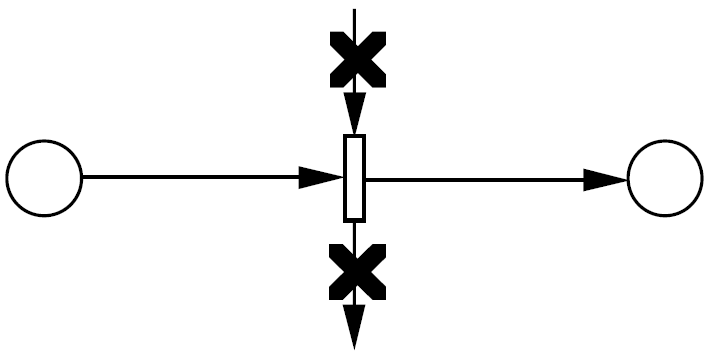
\includegraphics[width=0.25\linewidth]{./marco_teorico/redes_de_petri/img/Petri10}
			\caption{Ilustraci�n de la restricci�n para formar m�quinas de estados}
			\label{fig:Petri10}
		\end{figure}
		
		Generando un modelo con Redes de Petri que cumpla la restricci�n de la Ecuaci�n \ref{eq:petri_state_machine} es posible garantizar que el modelo cumple con todas las propiedades propias de las m�quinas de estado, es decir, es conservativa y acotada. La propiedad de vivacidad en este tipo de redes, es simple de demostrar y puede ser calculada de forma lineal con el algoritmo de Tarjan \cite{diaz_petri}.
	
	\subsection{Grafos de marcado}
	
		Para representar un grafo marcado con una Red de Petri debe cumplirse que: una plaza s�lo puede tener un �nico arco de entrada y un �nico arco de salida, las transiciones no tienen restricciones. De esta manera, si es posible que exista concurrencia y adem�s, no existen conflictos dado que un token solo puede disparar una transici�n.
	 
		Matem�ticamente, sea $p$ una plaza perteneciente al conjunto de plazas $P$ se tiene que:
		\begin{equation}
			\forall p\in P : \mid p\bullet \mid =\mid\bullet p \mid =1
			\label{eq:petri_grafo_marcado}
		\end{equation}
		
		\begin{figure}[H]
			\centering
			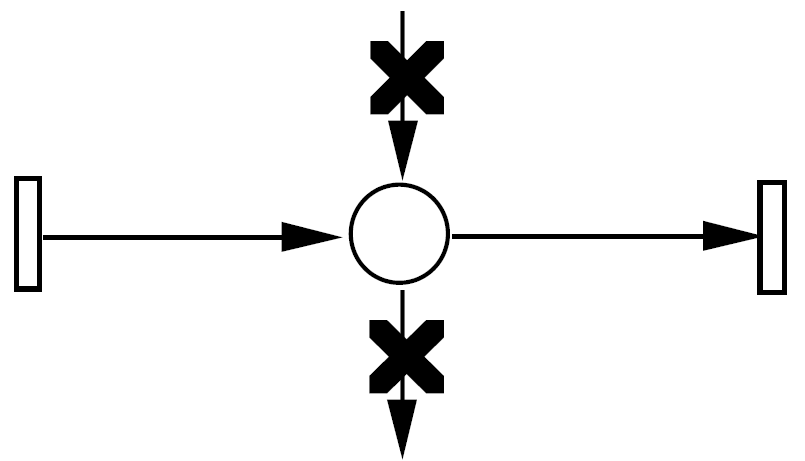
\includegraphics[width=0.25\linewidth]{./marco_teorico/redes_de_petri/img/Petri11}
			\caption{Ilustraci�n de la restricci�n para formar grafos de marcado.}
			\label{fig:Petri11}
		\end{figure}	
		
		Si la Red de Petri es de este tipo, la red es viva (sin deadlock) si y s�lo si cualquier circuito elemental de la red incluye un lugar que inicialmente estaba marcado \cite{diaz_petri}. Una red de este tipo, ser� estructuralmente limitada si es fuertemente conectada \cite{diaz_petri}.
	
	\subsection{Redes de libre elecci�n}
		
		En las redes de libre elecci�n, todo arco que va desde una plaza hacia una transici�n, es el �nico arco que sale desde esa plaza o es el �nico que entra en esa transici�n.
		\begin{equation}
			\forall p\in P : (\mid p\bullet \mid\leq 1) \vee (\mid\bullet(p\bullet) \mid =\{1\}
			\label{eq:petri_libre_eleccion}
		\end{equation}
		
		\begin{figure}[H]
			\centering
			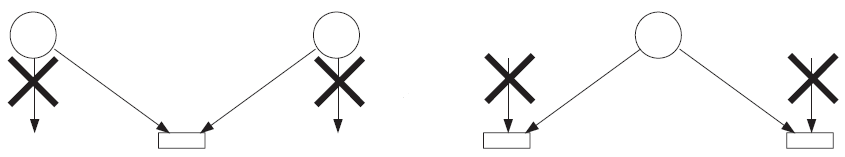
\includegraphics[width=0.7\linewidth]{./marco_teorico/redes_de_petri/img/Petri12}
			\caption{Red de elecci�n libre}
			\label{fig:Petri12}
		\end{figure}	
		
	\subsection{Redes de elecci�n libre extendidas}
	
		Si dos lugares tienen alguna transici�n de salida com�n, entonces ellos tienen todas sus transiciones de salida en com�n, matem�ticamente es equivalente a:
		\begin{equation}
			Sea\;p1\;y\;p2\in P: p1\bullet \cap p2\bullet \neq \phi \Rightarrow \mid p1\bullet \mid=\mid p1\bullet
			\mid
			\label{eq:petri_libre_extendida}
		\end{equation}

		\begin{figure}[H]
			\begin{center}
			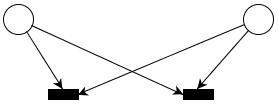
\includegraphics[width=0.3\linewidth]{./marco_teorico/redes_de_petri/img/Petri13}
				\end{center}
				\caption{Red de elecci�n libre extendida}
				\label{fig:Petri13}
		\end{figure}	
		
		De lo definido se puede notar que si una $t$ est� sensibilizada, todas las transiciones estar�n estructuralmente en conflicto. Por lo que se puede elegir libremente entre varias transiciones para disparar.
	  